% Author: Till Tantau
% Source: The PGF/TikZ manual
\documentclass[a4paper,11pt]{article}
\usepackage[utf8]{inputenc}
\usepackage{listings}
\usepackage{amsmath}    % need for subequations
\usepackage{graphicx}   % need for figures
\usepackage{verbatim}   % useful for program listings
\usepackage{color}      % use if color is used in text
%\usepackage{subfigure}  % use for side-by-side figures
\usepackage{hyperref}   % use for hypertext links, including those to external documents and URLs
\usepackage{url}
\usepackage{float}
\usepackage{todonotes}
\usepackage{tikz}
\usepackage{enumitem}
\usepackage{hyperref}
\usepackage{pdfpages}
\usepackage{caption}
\usepackage{epsfig}
\usepackage{subcaption}
\usepackage{listings}
\usepackage{color}
\usepackage{amsfonts}
\usepackage{latexsym}
\usepackage[T1]{fontenc} % use for allowing < and > in cleartext
\usepackage{fixltx2e}    % use for textsubscript
\usepackage[linesnumbered,boxed,ruled]{algorithm2e}
\usepackage{mathtools}
\DeclarePairedDelimiter{\ceil}{\lceil}{\rceil}
% \newcommand{\BigO}[1]{\ensuremath{\operatorname{O}\left(#1\right)}}
\newcommand{\BigO}[1]{\ensuremath{\mathop{}\mathopen{}\mathcal{O}\mathopen{}\left(#1\right)}}

\definecolor{mygreen}{rgb}{0,0.6,0}
\definecolor{mygray}{rgb}{0.5,0.5,0.5}
\definecolor{mymauve}{rgb}{0.58,0,0.82}
\lstset{ %
  backgroundcolor=\color{white},   % choose the background color; you must add \usepackage{color} or \usepackage{xcolor}
  basicstyle=\footnotesize,        % the size of the fonts that are used for the code
  breakatwhitespace=false,         % sets if automatic breaks should only happen at whitespace
  breaklines=true,                 % sets automatic line breaking
  captionpos=b,                    % sets the caption-position to bottom
  commentstyle=\color{mygreen},    % comment style
  deletekeywords={...},            % if you want to delete keywords from the given language
  escapeinside={\%*}{*)},          % if you want to add LaTeX within your code
  extendedchars=true,              % lets you use non-ASCII characters; for 8-bits encodings only, does not work with UTF-8
  %frame=single,                    % adds a frame around the code
  keepspaces=true,                 % keeps spaces in text, useful for keeping indentation of code (possibly needs columns=flexible)
  keywordstyle=\color{blue},       % keyword style
  language=Octave,                 % the language of the code
  morekeywords={*,...},            % if you want to add more keywords to the set
  numbers=left,                    % where to put the line-numbers; possible values are (none, left, right)
  numbersep=5pt,                   % how far the line-numbers are from the code
  numberstyle=\tiny\color{mygray}, % the style that is used for the line-numbers
  rulecolor=\color{black},         % if not set, the frame-color may be changed on line-breaks within not-black text (e.g. comments (green here))
  showspaces=false,                % show spaces everywhere adding particular underscores; it overrides 'showstringspaces'
  showstringspaces=false,          % underline spaces within strings only
  showtabs=false,                  % show tabs within strings adding particular underscores
  stepnumber=2,                    % the step between two line-numbers. If it's 1, each line will be numbered
  stringstyle=\color{mymauve},     % string literal style
  tabsize=2,                       % sets default tabsize to 2 spaces
  %title=\lstname                   % show the filename of files included with \lstinputlisting; also try caption instead of title
}

\bibliographystyle{plain}
\begin{document}
\graphicspath{ {./images/} }
\date{May 21st 2014}
\title{Similarity Filters\\A Survey}

\author{Marcus Gregersen\\
\texttt{mabg@itu.dk}
\and Martin Faartoft\\
\texttt{mlfa@itu.dk}
\and Rick Marker\\
\texttt{rdam@itu.dk}}
%TODO vejleder og institut
\clearpage\maketitle
\thispagestyle{empty}
\setcounter{page}{1}
\begin{abstract}
The abstract goes here
\end{abstract}

\newpage
\setcounter{page}{1}

\section{Introduction}
In the following we investigate the Similarity Search problem. Different approaches have been explored by earlier work, and in this paper we will investigate two of those; 'Distance-Sensitive Bloom Filters'\cite{paper:harvard} by Kirsch and Mitzenmacher, and 'Locality-Sensitive Bloom Filter for Approximate Membership Query'\cite{paper:hua} by Hua et al.

\subsection{The Problem}
The Similarity Search problem can be stated as follows: Given a set of elements $S$, determine if there exists an element $s \in S$ that is 'close' to a given query element $q$. Where 'close' is defined as being within a given distance, $d$ using a certain metric.

%Real world example
A real-word example could be a database of candidates used by a headhunting agency. Each candidate in the database would then have a set of attributes, for example \{\texttt{age}, \texttt{gender}, \texttt{race}, \texttt{education}, and \texttt{experience}\}.
An application of Similarity Search can then be formulated as: "Given some person P, does the database contain one or more candidates, similar to P?"

% Begræns problemet
In the following we consider the Similarity Search problem for bit-vectors of length $l$, and Hamming distance as metric. This reduction maintains a high degree of generality, since elements from many domains can be encoded as bit-vectors.

\subsection{Definitions}
\begin{description}
\item \textbf{Hamming distance}

A distance metric for bit-vectors. The Hamming distance between two vectors $v_1, v_2$ is given as the number of positions $i$ where $v_1[i] \neq v_2[i]$

\item \textbf{Bloom Filter}

In 'An Improved Construction for Counting Bloom Filters' \cite{paper:bloom} Bloom filters are described as:
\begin{quotation}
A Bloom filter is an inexact representation of a set that allows for false positives when queried; that is, it can sometimes say that an element is in the set when it is not. In return, a Bloom filter offers very compact storage: less than 10 bits per element are required for a 1\% false positive probability, independent of the size or number of elements in the set.
\end{quotation}


\item \textbf{Locality-Sensitive Hashing}
\label{sec:lsh}

Ordinary hashing tries to minimize the probability of a collision, while Locality-Sensitive Hashing (LSH) attempts to maximize the collision probability for sufficiently similar elements.

LSH functions are not known for all similarity-measures, but for Hamming distance on bit-vectors, a particularly simple one is known.
Sample a fixed number of bit positions, $l'$, from the input bit-vector, uniformly at random. This LSH now considers all vectors that are identical on the $l'$ sampled bit positions, identical. This type of collision is desired (called locality collision in the following). Storing all of these requires $2^{l'}$ space, which is not feasible for large values of $l'$. The solution is to interpret the bit vector as an integer, and store that value in some array of size $m$. since $m < 2^{l'}$, we have from the pigeonhole principle, that multiple integers must hash to the same value. This type of collision is not desirable, and leads to an increase in false positives. We call this an accidental collision in the following.

\item \textbf{$\epsilon$-closeness}
  \begin{itemize}
    \item If an element $s \in S$ differs from $x$ in at most an $\epsilon$-fraction of the bits, it is said to be $\epsilon$-close to $x$. The data structure must return “close”.
    \item If every vector $s \in S$ differs from $x$ in at least a $\delta$-fraction of the bits, then the data structure should return 'not close'.
    \item In all other cases, i.e. when the distance to the nearest vector is between $\epsilon$ and $\delta$, the data structure can give any answer it likes.
  \end{itemize}

\end{description}

\subsection{Naïve Approaches}
\label{naive_approaches}

\paragraph{Brute force}
The most obvious idea for solving the Similarity Search problem, is brute force. Store the elements $S$ in a linked list. When a query is made, simply scan the linked list, and calculate the distance from each element $s \in S$ the query element $q$. If $s$ satisfies the distance requirement, a match has been found. If the end of the linked list is reached, no match exists.

This will give a correct answer, and will work well for small problem instances, But the linear requirement on time and space in the total number of bits in $S$, is prohibitively expensive for many real-world applications. \todo{flet lidt om jobkandidat IRL snask ind her}

\paragraph{Bloom filters} If we relax the requirements on space or time, we can change these characteristics to support either constant-time queries, or space-efficiency, but not both.

While keeping in mind that standard Bloom filters only answer exact membership, we see that one way of achieving this is by relying on extra insertions. Everytime an element is added to the Bloom filter, all elements within distance $d$ are generated and added in addition to the original element.

Another way to go around this is by sacrificing time. This can be done by still doing normal insertions but instead querying for all elements with distance $d$ of the element we are comparing to. This approach has the benefit of still being space efficient but will cause an exponential blowup of the running time.


%     False Negatives (skal det være her?)



\section{Related work} % Ideer fra related works

\subsection{Distance-Sensitive Bloom Filters}
Kirsch and Mitzenmacher propose in the paper 'Distance-Sensitive Bloom Filters'\cite{paper:harvard} a novel way of using Bloom filters. The aim is to expand upon classical Bloom filters, enabling them to answer the question: "Does a set contain an element similar to a given element?". They note that such a data structure has a number of practical uses, if it can be made sufficiently effective in both time and space.

The way they accomplish this is by using locality sensitive hashing algorithms (TODO REF), such that two elements that are sufficiently similar will, with a high probability, hash to the same value. They also use a partitioned Bloom filter, which is a like a standard Bloom filter except each locality sensitive hashing algorithm maps into its own bit array, instead of all the hashing algorithms share the same bit array.

When querying the Bloom filter for an approximate match, the element is hashed with all the hashing algorithms, and the corresponding indiceses are checked. If there are more bits, than a specified threshold (T), that is set to 1, it returns that the data contains an element that is close to the query element. The use of a threshold is the reason why it is possible to have false positives using this data structure.

A disadvantage to this approach, compared to a classical Bloom filter, is that it introduces the possibility of false negatives.

In their experiments they manage to achieve false postive rates and false negative rates of 1.5\% and 0.2\% respectively for 1000 elements, and 0.016\% and 0.003\% for 1000. For 1000 elements they use 64\% of the total space of the elements, and for 10000 elements they use 51\% of the total space.



\subsection{Locality-Sensitive Bloom Filter for Approximate Membership Query}
The paper written by Hua et al.\cite{paper:hua}, takes a slightly different approach than \cite{paper:harvard}. They use a standard Bloom Filter data structure, with LSH functions in place of ordinary hash functions, but no thresholding. They call this a 'Locality Sensitive Bloom Filter'. This 'naive' approach, has a high probability of both false positives and false negatives.

% Rick: Skal nok omskrives.. Er ikke selv helt tilfreds
In the report they have chosen to use a 'proximity measure', which makes it impossible to compare the results to the ones found in \cite{paper:harvard} directly and all data presented is only available through graphs. From the graphs, however, we can see that they achieve between 85\% and 100\% accuracy.

\paragraph{Minimizing False Positives}
Every time an element $q$ is checked for approximate membership, the LSBF is checked. If every bit in the array that $q$ hashes to is set to $1$, that could mean one of two things.
1) An element $p$ exists in the LSBF, that is approximately close to $q$ (a true positive)
2) Multiple elements added to the LSBF, together, have conspired to set the all the bit positions corresponding to $q$ to $1$, and no single element is approximately close to $q$. (a false positive).

To minimize the probability of a FP, a Verification Scheme (VS) data structure is added.
This is a standard Bloom filter (ordinary hashing, not LSH), and is maintained as follows: Every time an element is added to the LSBF, the bit positions that corresponds to that element, are encoded (see figure \ref{fig:verification_scheme}) and inserted into the VS Bloom filter.
Now when the LSBF is queried, it first verifies that all bits corresponding to the query element $q$ are set to $1$ in the LSBF, and then encodes the bit positions (figure \ref{fig:verification_scheme}), and queries the VS for an exact match. If an exact match for the encoded version of $q$ is found in VS, then it is highly likely that a single element $p$ is responsible for setting all the bits in the LSBF, and the query will return a 'yes'. If, on the other hand, the VS does not contain an element that matches the encoded $q$, then multiple elements must be responsible for the bits being set, and the query will return 'no', effectively catching a false positive.

\begin{figure}[H]
\centering
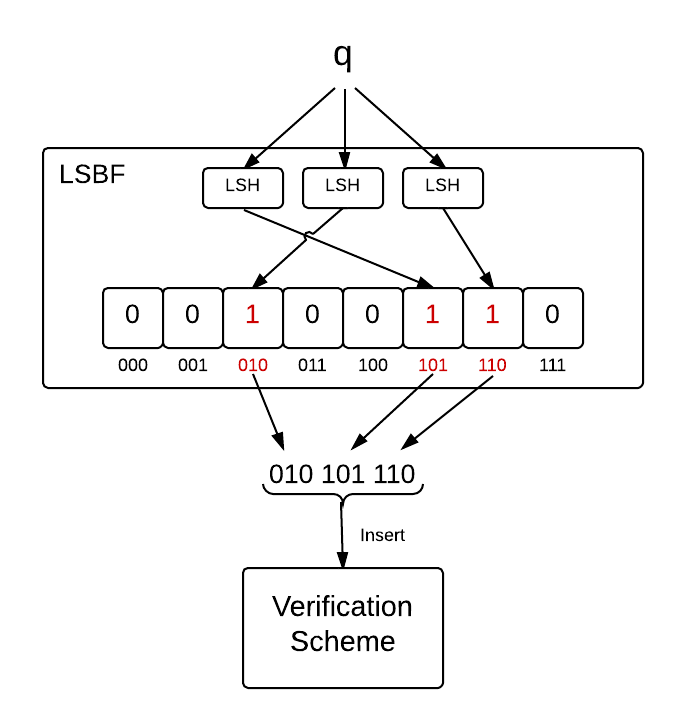
\includegraphics[width=.5\linewidth]{verification_scheme}
\caption{Maintaining the Verification Scheme, when adding elements to an LSBF}
\label{fig:verification_scheme}
\end{figure}


Note that the VS is a standard Bloom filter, and therefor allows false positives itself. That means it only serves to minimized false positives, not outright remove them.

\paragraph{Minimizing False Negatives}
They use a method called Active Overflowed Scheme, which utilizes the property of the locality sensitive hashing algorithms that proximate elements will be stored close to each other. The idea is that a pair of close elements may not be hashed to the same value, but instead be put in adjacent bins in the bit array. So when querying, instead of just looking at the bits which represents the hashed element, you also check the $t$ closest bits to either side. $t$ will depend on the price of false positives compared to false negatives as this approach will introduce more false positives.

We have based our work on the work of Kirsch and Mitzenmacher, as their work seems more robust by using thresholds and the way they present their results allow for easier comparison with our results. They main reason we have not used Hua et al. in our work is that they rely a lot on their LSHs, but provide no clear description on how they construct these. Furthermore, it is unclear how they are able to implement a data structure in which they efficiently are able to store data for their Active Overflowed Scheme. As this seems to be the basis for half of their contribution, and along with the fact that their results are in a format which makes them hard to compare against, we have chosen not to include them in our work

\section{Theory} % Dette afsnit skal nok hedde noget andet

%valg af T, k, m', n', n
  %pulje af hashfunktioner (seed til random generator)
  %beregn true/false positives og true/false negatives
%find epsilon og sigma fra ovenstående
%diskutér false positives (sandsynlighed)
%diskutér false negatives (kan de elimineres?)



\section{Experiments}
\todo{Det kunne være mere interesseant at have antal bits på x-aksen.}
\begin{figure}[H]
\centering
\begin{subfigure}{.5\textwidth}
  \centering
  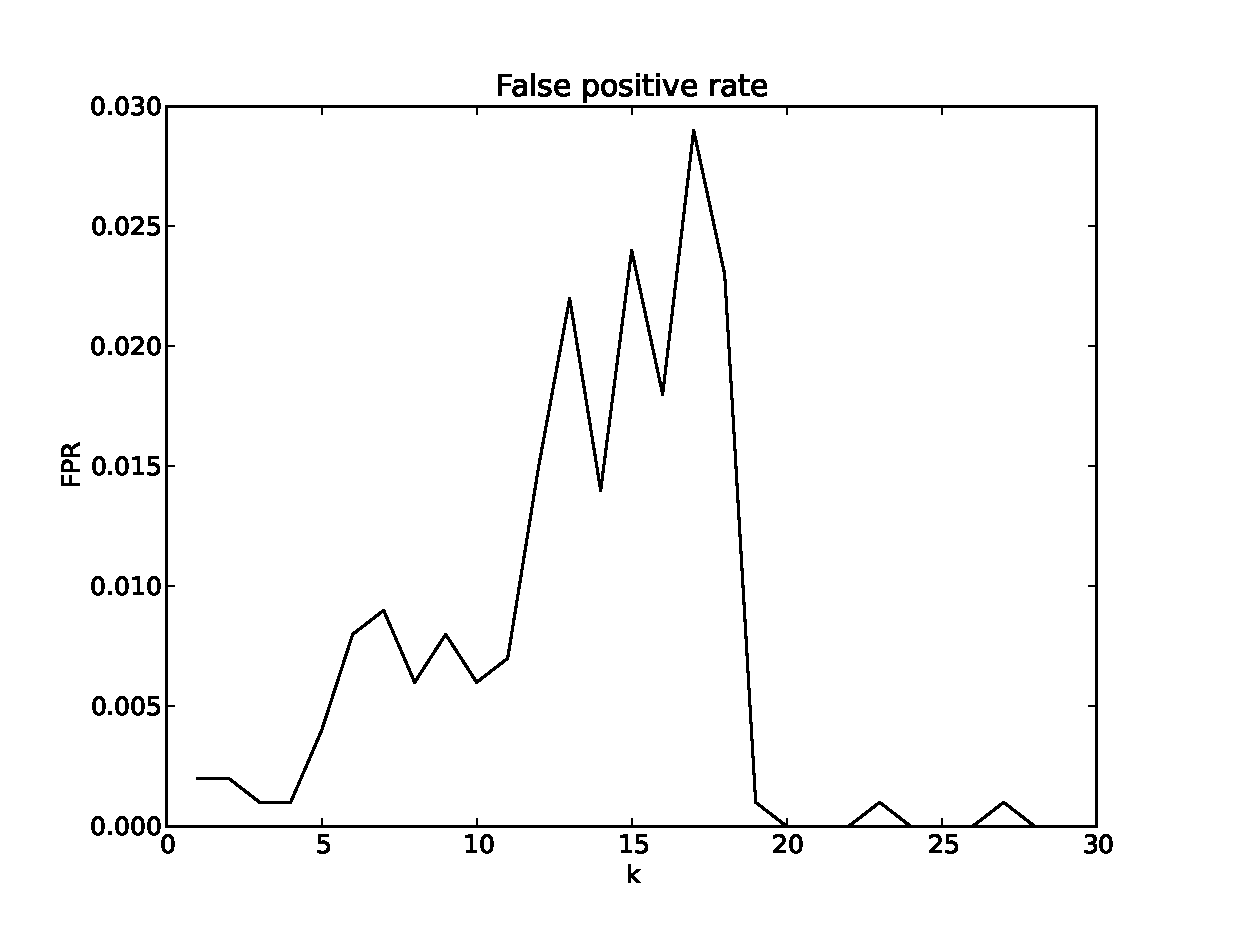
\includegraphics[width=.95\linewidth]{FPR1}
\end{subfigure}%
\begin{subfigure}{.5\textwidth}
  \centering
  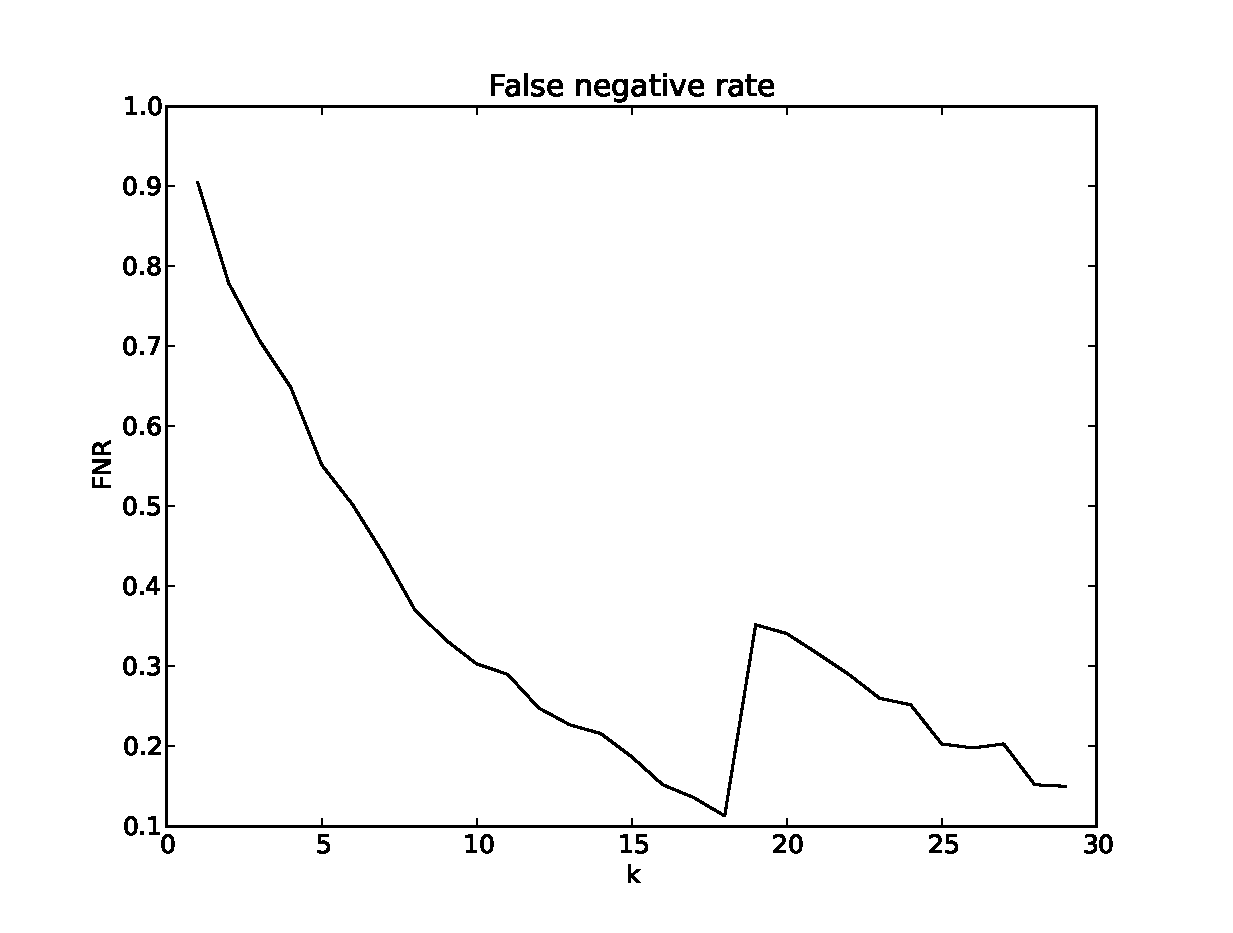
\includegraphics[width=.95\linewidth]{FNR1}
\end{subfigure}
\caption{The observed false positive and false negative rates for $n$ = 1000, $l$ = 65536, $\epsilon$ = 0.1, and $\sigma$ = 0.4}
\label{fig:n1000}
\end{figure}
\begin{figure}[H]
\centering
\begin{subfigure}{.5\textwidth}
  \centering
  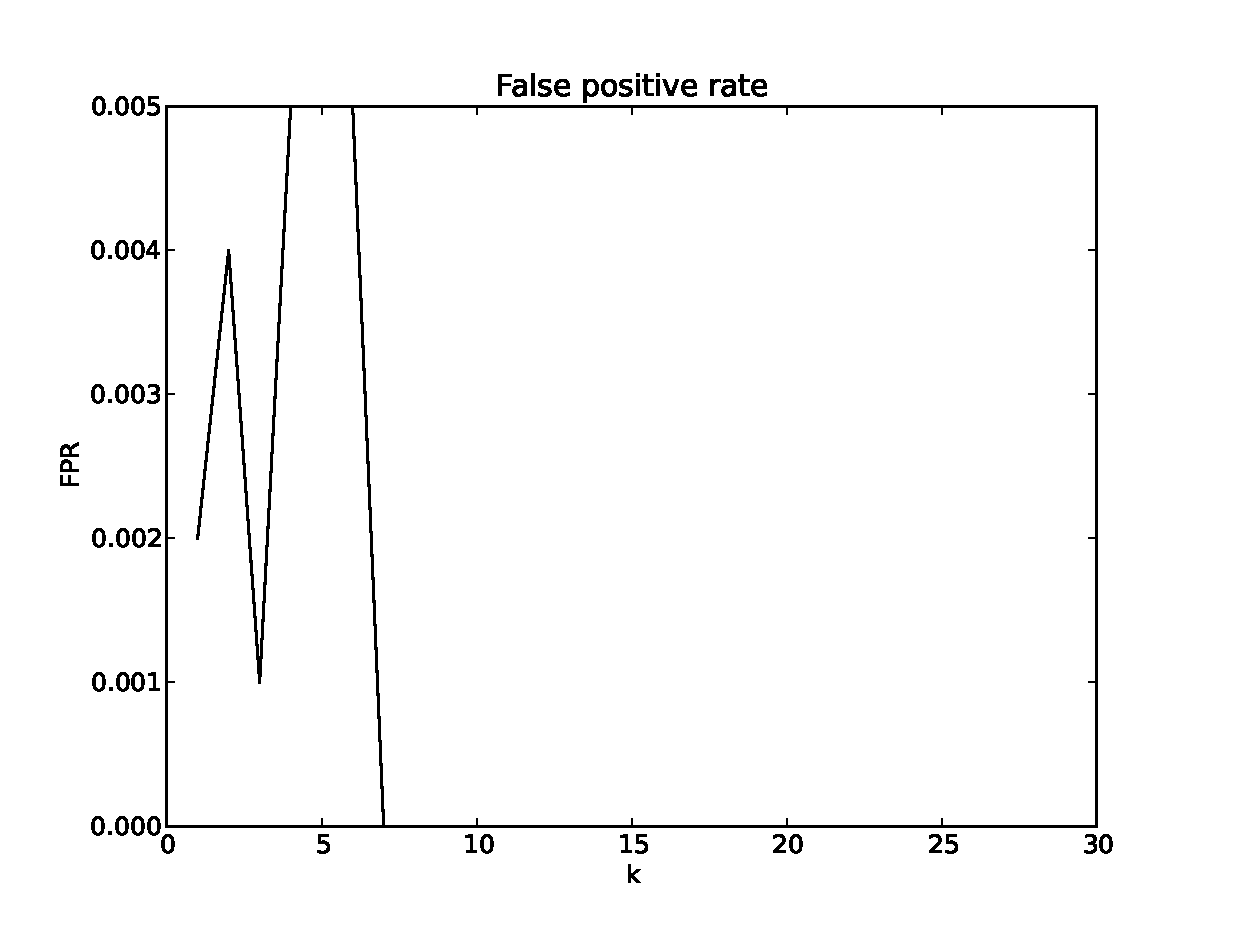
\includegraphics[width=.95\linewidth]{FPR2}
\end{subfigure}%
\begin{subfigure}{.5\textwidth}
  \centering
  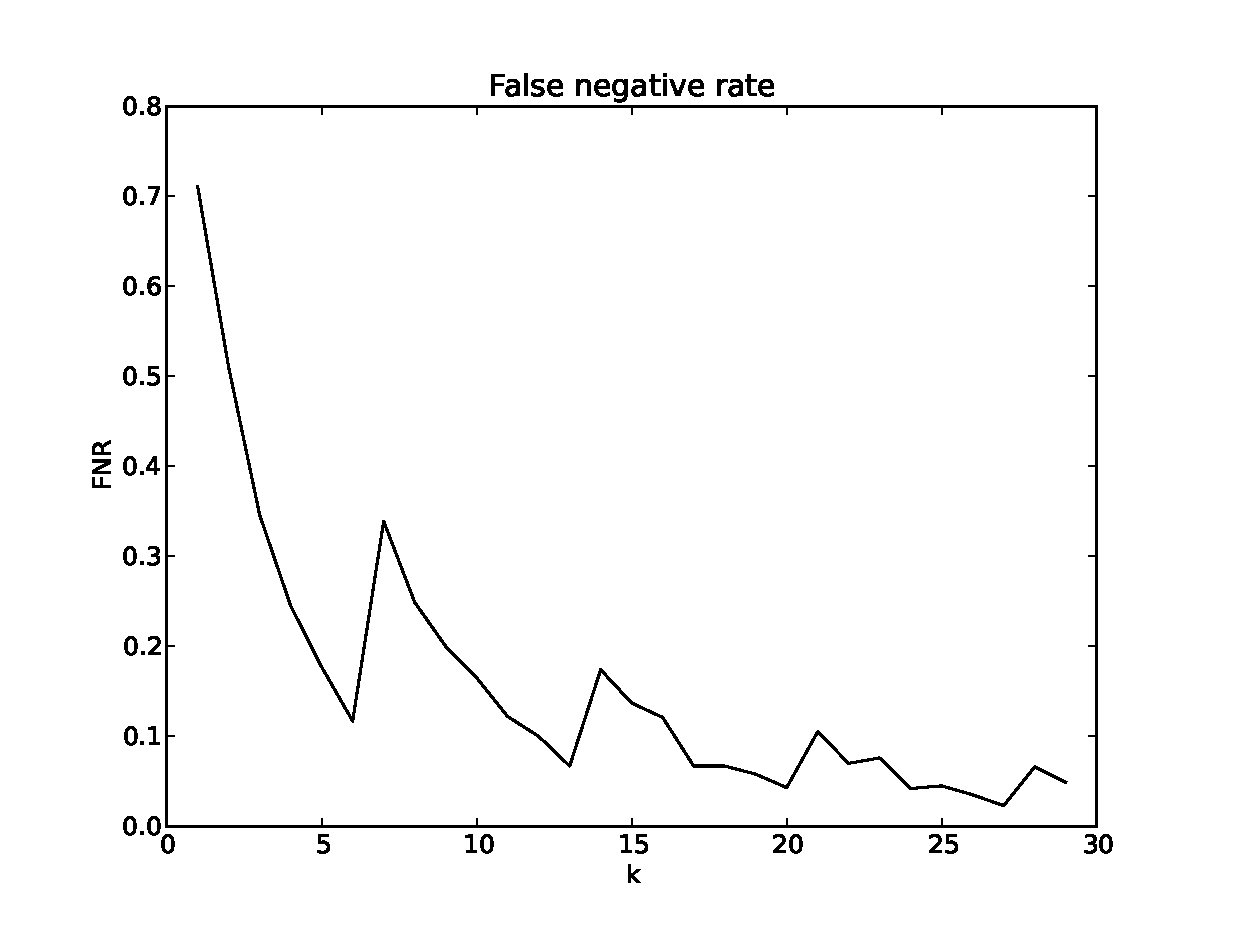
\includegraphics[width=.95\linewidth]{FNR2}
\end{subfigure}
\caption{The observed false positive and false negative rates for $n$ = 10000, $l$ = 65536, $\epsilon$ = 0.05, and $\sigma$ = 0.4}
\label{fig:n10000}
\end{figure}

%tegn nogle grafer

% Forsøg at finde variable eksperimentelt
% Forsøg at variér closeness/farness i kandidater og tegn FP og FN-rate som funktion af disse

\section{Suggested Improvements}
In the following, we present our contributions. They take the form of a series of suggested improvements and ideas for alternate usage.

\subsection{Balanced LSH Bit Sampling} \label{sec:balanced}
The default way to initialize the LSH functions used in the Distance-Sensitive Bloom filter (DSBF), is for each of the $k$ LSH functions, to choose $l'$ bit positions to sample, uniformly at random. On average this should spread the sampled bits out nicely across the k hash-functions, but in some cases this will result in a skewed distribution, meaning that some bits are oversampled, while others may not be sampled at all. This skew will degrade the performance of the DSBF, resulting in more false answers.
\\
This can be remedied, by initializing the LSHs such that all bit positions are sampled equally often.
In practice we do this by first preparing a vector of length $k \cdot l'$ by repeating the the integers from 0 to $l$ as many times as required. We then shuffle the vector, and assign each of the $k$ functions a sub-vector of length $l'$, making sure that every index in the sub-vector is unique. This preprocessing step takes $O(l)$ time, and protects the DSBF from poor performance due to skewed sampling.

Figure TODO shows an experiment run with Balanced bit sampling enabled (TODO some color) and disabled (TODO some other color), and shows that this optimization in some cases improves the performance of the DSBF, but never degrades it.
\todo{produce and insert graphs here}

\subsection{Eliminating False Negatives}
Building on the previous idea from \ref{sec:balanced}, we suggest a way to eliminate false negatives from the DSBF data-structure.

\paragraph{False Negatives} \label{p:fn}happen when a query element is within distance $\epsilon$ of an element in S, but is reported as being 'not close'. This happens when too many of the $k$ LSH functions report false, driving the number of trues below the threshold $t$. We know that each of the LSHs that report false, will sample at least one bit in which $q$ and every element $s \in S$ differ. Since q, by definition, is 'close' to some element $s \in S$, the maximum number of differences between $q$ and the closest element in $S$ is: $\epsilon_{abs} = \ceil{\epsilon \cdot l}$, where $l$ is the element length. Assuming that each is sampled an equal number of times (ensured by \ref{sec:balanced})): $l_n = \ceil{\frac{k \cdot l{'}}{l}}$, the maximum number of hash-functions that can report false is: $n_{false} = e_{abs} \cdot l_n$.

\paragraph{Providing a guarantee} against false negatives can be achieved by lowering the DSBF threshold appropriately. Armed with the knowledge of $n_{false}$ from \ref{p:fn}, we can set $t = k - n_{false}$, and thereby eliminate the possibility of false negatives completely.

Lowering $t$ comes at a price, the lower the value of $t$, the higher the probability of a false positive. In the edge case, where $t=0$, the DSBF becomes useless, answering 'close' to every query. Taking this into account, we have to constrain the value of $n_{false}$ such that $t>0$.
\[t > 0 \leftrightarrow k > n_{false} \leftrightarrow k > \epsilon_{abs} \cdot l_n\]
This turns out to be a big deal, $k$ is usually below 100, $l_n$ can be kept small, but not smaller than 1. Those two bound $\epsilon_{abs}$, to definitely be below 100, which in turn makes it impossible for $\epsilon$ to be a constant fraction of $l$, for increasing $l$ values.

\subsection{Wildcard Search}
The DSBF structure can, as we have seen, be used to answer questions of the form "does $S$ contain an element that is 'close' to $q$". In the following. A natural extension to this, is to want to ignore certain bits in $q$, when calculating the similarity.

If we examine the job applicants example from the introdution, one application of the Similarity Search with Wildcards can formulated as: Given some employee with the attributes \{\texttt{age}, \texttt{gender}, \texttt{race}, \texttt{education}, \texttt{experience}\} does the dataset contain one or more applicants that match on at least two attributes while disregarding the attributes \texttt{gender} and \texttt{age}?.

\subsubsection*{The Extended Problem}
The extended problem can be stated as follows:

Let $W$ be a set of wildcard bit positions: $\forall w \in W (w \in \mathbb{Z}^+ \land w < l)$.\\
Given a set of elements $S$, a query element $q$ and a set of wildcards $W$. Determine if there exists an element $s \in S$ that is 'close' to $q$, not counting differences on wildcard positions $W$. Where 'close' is defined as being within a given distance, $d$ using a given metric.

\subsubsection*{Solving Wildcard Search}
We have identified two approaches to solving the extended problem.
\paragraph{The first approach} is to simply ignore the output from all LSH's that sample one or more wildcard bits. This can be done without modifying the insertion of elements into the DSBF, and without storing additional data. However, it raises some troublesome questions.

\begin{itemize}
\item How should the threshold be chosen, when the number of ignored LSH's changes from query to query?
\item How should the bits to sample for each LSH be chosen, to minimize the probability that the LSH's that are ignored due to wildcarding, are not the only ones sampling some bit position $p \notin W$?, accidentally ignoring $p$ when counting differences.
\end{itemize}

The second question intuitively seems like it will require $|W|$ to be small, in order to keep the false positive rate low. And overall, the approach seems inferior to the second approach.

\paragraph{The second approach} is to use the idea from the naïve solution, outlined in \ref{naive_approaches} and query the DSBF structure multiple times with different variations of $q$. As a simple example, assume that we are querying a previously constructed DSBF with the following:
\[q=[0,0,0,0], W=\{2,3\}\]
Since the last two bits are wildcarded, we generate all possible variations of $q$ on the wildcarded positions:
\[q_1=[0,0,0,0], q_2=[0,0,0,1], q_3=[0,0,1,0], q_4=[0,0,1,1]\]
We now query the DSBF with each of the variations, and if any of them returns 'close', we report 'close' to the original query $q, W$.

This requires $2^{|W|}$ queries in the worst case, and half \todo{det med half gælder kun hvis vi ved at den er close}of that in the average case, assuming we stop querying after receiving the first 'close' response. Using this approach, the time complexity for a query with wildcards is exponential in the number of wildcarded bits.\\

This result is reasonably good for a small number of wildcards, but we can do better if we leverage the inner workings of the DSBF, instead of treating it as a black box.
When the DSBF is queried, it hashes the query element $q$ using $k$ different LSH functions, and checks the corresponding locations in the internal memory. Each of the $k$ LSH functions sample a different subset $l'$ out of the total $l$ bits in $q$. This means that when the DSBF is queried multiple times with different variations of $q$, some of the LSH functions will do repeated work if they do not sample any of the wildcarded bits.

We wish to eliminate this repeated work. Assume again the simple example:
\[q=[0,0,0,0], W=\{2,3\}\]
Additionally assume that the DSBF contains 3 LSH functions that sample bits as follows:
\[B_{LSH_1}=\{0,1\}, B_{LSH_2}=\{1,2\}, B_{LSH_3}=\{2,3\}\]
Instead of querying the DSBF multiple times, we push that one level down, querying each LSH (possibly) multiple times.
$LSH_1$ receives $q$ and $W$. It calculates $B_{LSH_1} \cap W = \emptyset $, meaning that it samples none of the wildcarded bits. It then simply hashes $q$, and returns the corresponding value from memory.
$LSH_2$ calculates $B_{LSH_2} \cap W = \{2\}$. It then generates all possible variations of $q$ on the sampled wildcard positions:
\[q_1=[0,0,0,0], q_2=[0,0,1,0]\]
looks up the corresponding positions, and returns the binary 'OR' between the values.
$LSH_3$ does the same thing, but since it samples both bits 2 and 3, it has to generate 4 variations of $q$ and 'OR' the results.
The rest of the query is unchanged, if the number of LSH's that returned 'true' exceeds the threshold, $t$, the DSBF reports 'close'.\\

The above requires $2^{min(|W|, l')}$ queries in the worst case.
This is an improvement in two ways: The worst-case time complexity is now upper bounded by $2^{l'}$, and more importantly the average time complexity is significantly improved, since the worst-case now only happens when an LSH hashes all the bit positions in $W$.
\todo{analyse af average case time complexity goes here?}

%advantages
%no prior knowledge of W required
%no changes to insert
%no extra memory required
\subsubsection*{Properties of Wildcard Search}
The second approach has the following desirable properties:
\paragraph{No prior knowledge of W required} At the time of construction, the DSBF requires no knowledge of what / how many bits will be wildcarded.

\paragraph{No changes to 'insert'} The process of adding items to the DSBF does not require modifications to support wildcard search.

\paragraph{No additional memory required} Because the wildcard search uses multiple queries, no additional memory is required.
\\
%drawbacks
%increased query time-complexity
%increased FP due to non-LSH collisions

And the following undesirable properties:
\paragraph{Increased Time Complexity for Wildcard Search} Multiple queries for each LSH, means that the time complexity is no longer constant.

\paragraph{Increased False Positive Rate} When querying each LSH multiple times, the chances of a false positive also increases. The probability of an accidental collision\footnote{See Section \ref{sec:lsh}} is constant, so querying multiple times will increase the probability of a false positive.

%experiments



\section{Conclusion}
\newpage

\begin{thebibliography}{}

\bibitem{paper:harvard}
Adam Kirsch, Michael Mitzenmacher
"Distance-Sensitive Bloom Filters"

\bibitem{paper:hua}
Yu Hua, Bin Xiao, Bharadwaj Veeravalli, Dan Feng, "Locality-Sensitive Bloom Filter for Approximate Membership Query", IEEE Transactions on Computers, Vol. 61, No. 6, 2012


\bibitem{paper:bloom}
Flavio Bonomi, Michael Mitzenmacher, Rina Panigrahy, Sushil Singh, and George Varghese
"An Improved Construction for Counting Bloom Filters"

      %Sådan her ref'er man en URL
      %\bibitem{lit:json}
      %\url{http://tools.ietf.org/html/rfc4627}
      %Retrieved: 2013-05-02
\end{thebibliography}

%code in appendix
\section*{Appendix}
%\lstinputlisting[language=Python]{../tools/size_estimator.py}


\end{document}
